% REAL - ICSE 2027 Tool Demonstration track. Skeleton (task D2, 2026-10-08).
% Format required by the call: IEEEtran, 10pt, conference; no compsoc options;
% <= 4 pages INCLUDING references, figures, tables, appendices; authors named
% (single-anonymous); the abstract ends with the video URL.
% Page budget (approx.): abstract 0.2 | 1 intro 0.5 | 2 background 0.2 |
% 3 tool + Fig. 1 + Fig. 2 1.2 | 4 case study + Table 1 1.0 | 5 limits/study/carbon 0.25 |
% 6 related 0.2 | 7 availability 0.1 | references 0.6  (= 4.25: trim background first)
\documentclass[10pt,conference]{IEEEtran}
\usepackage{graphicx}
\usepackage{booktabs}
\usepackage{url}
\usepackage{cite}
\usepackage{xcolor}
\newcommand{\todo}[1]{\textcolor{red}{[TODO: #1]}}

\begin{document}

\title{REAL: A Tool for Failure-Driven Requirements Engineering\\of Machine-Learning Systems}

% TODO D1: authors, order, affiliations, ORCIDs (single-anonymous: names are shown)
\author{\IEEEauthorblockN{\todo{Author 1}}
\IEEEauthorblockA{\todo{Affiliation}\\\todo{email}}
\and
\IEEEauthorblockN{\todo{Author 2}}
\IEEEauthorblockA{\todo{Affiliation}\\\todo{email}}}

\maketitle

\begin{abstract}
% ~150 words: problem, tool, what it automates beyond the research paper,
% case study result, availability. MUST end with the video URL.
Testing machine-learning systems yields failures, but not what to change:
the data, the model, the system around it, the requirement, or the
assumptions about the world. \todo{Tool sentence.} \todo{What it automates:
validity from the requirement's own assumptions, obstacle analysis,
recorded decisions, labelled revision.} \todo{Case study: automated braking on
CARLA, N rounds, key result.} \todo{Availability: Docker demo, DOI.}
Video: \url{\todo{YouTube URL}}
\end{abstract}

\section{Introduction}
% 0.5 page. MUST name the envisioned users and the SE challenge (call).
\todo{Challenge: failures pile up with no link back to requirements; validity
and obstacle analysis are manual; decisions are not recorded.}
\todo{Users: requirements engineers and ML/AV engineers deciding what to
change; assurance reviewers who need the trail.}
\todo{Gap: the REAL framework~\cite{real2026} defines the loop and does failure
grouping and validity by hand; no tool exists.}
\todo{Contributions (3), each beyond the research paper:
(1) validity computed from the requirement's own domain assumptions, with
per-assumption verdicts and refusal of assumptions about the system;
(2) automated obstacle analysis and a cross-layer mitigation menu;
(3) recorded human decisions turned into a labelled requirement revision
([S]/[R]/[D]/[T]) with run provenance, and honest analysis (masked vs
resolved, failure-mode shift, scene defects, search-sampling caveat).}

\section{Background: REAL in Brief}
% 0.2 page. D,S |= R; valid vs spurious; obstacles; the loop. No new theory.
\todo{Zave and Jackson~\cite{zave1997}; KAOS obstacles~\cite{lamsweerde2000};
REAL's Identify--Analyse--Mitigate loop~\cite{real2026}.}

\section{The REAL Tool and Its Workflow}
% 1.2 pages incl. Fig. 1 (architecture/workflow) and Fig. 2 (review page).
% The call asks for the workflow required of users: make it a numbered list.
\begin{figure*}[t]
\centering
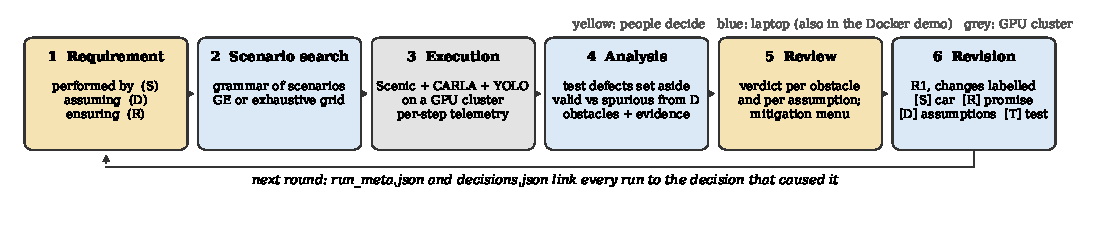
\includegraphics[width=\textwidth]{figures/fig1_workflow.pdf}
\caption{REAL's loop as implemented by the tool. People write the requirement and
decide (yellow); search, analysis and revision run on a laptop and in the Docker
demo (blue); scenarios execute in CARLA on a GPU cluster (grey). Every run is linked
to the decision that caused it. (Regenerate: \texttt{figures/make\_fig1.py}.)}
\label{fig:arch}
\end{figure*}
\subsection{Requirement language}
\todo{performed by (S), assuming (D), ensuring (R soft goals); refusal of
assumptions about the car; example from R\_baseline.dsl.}
\subsection{Scenario search and execution}
\todo{Grammar; grammatical evolution~\cite{oneill2001,grape2022} over 21,120
scenarios, deliberately beyond the assumptions; Scenic~\cite{scenic2023} and
CARLA~\cite{carla2017}; per-step telemetry; on-road and crossing checks.}
\subsection{Validity and obstacles}
\todo{held / broken / not measured; load-bearing verdicts; failure types;
obstacles with evidence; mitigation menu across data, model, system,
requirement.}
\subsection{Review and revision}
\todo{5-screen review page (Fig. 2); decisions.json; labelled diff; provenance.}
\subsection{Reproducibility}
\todo{run metadata, one-change comparison, pre-registered predictions,
laptop scene check, GE sampling caveat + grid check, Docker demo.}

\section{Case Study: Automated Braking}
% 1.0 page incl. Table 1. Every number from docs/paper/numbers.md (task B10).
\begin{table}[t]
\centering
\caption{Rounds of the loop. \todo{fill from the run folders}}
\label{tab:rounds}
\begin{tabular}{@{}llrrl@{}}
\toprule
Round & Change & Fail. & Stalls & Supported obstacles \\
\midrule
1 & baseline (emergency braking) & 76\% & 12 & DetectionTooLate, \ldots \\
2 & [S] proportional braking & 3\% & 113 & StandoffUnnecessaryStop \\
2b & [T] fixed scene & \todo{} & \todo{} & \todo{} \\
GE & search beyond D0 & \todo{} & \todo{} & \todo{} \\
3 & [D][R][S] & \todo{} & \todo{} & \todo{} \\
\bottomrule
\end{tabular}
\end{table}
\todo{The failure-mode shift (round 2); the scene defects the tool led us to
([T]); rounds 1--2 re-judged under the baseline assumptions; run 2b; GE and
its grid check; round 3; differences from the research paper.}

\section{Limitations, Planned Study, Carbon Footprint}
% 0.25 page. Planned study design (call: early prototypes) + pilot if done.
\todo{Simulator fidelity; one learned component; judgement-call support bars;
small trial counts; GE sampling bias; authors as reviewers.}
\todo{Planned practitioner study: design. Pilot (E8) if done.}
\todo{Carbon: GPU-hours $\times$ A100 power $\rightarrow$ kWh, CO$_2$e; the demo
needs no GPU.}

\section{Related Tools}
% 0.2 page.
\todo{Scenic/VerifAI falsification~\cite{viswanadha2021}; DYNASTO~\cite{dynasto2026};
failure models for spurious failures~\cite{jodat2024}; Anunnaki~\cite{anunnaki2024}.
Difference: REAL closes the loop to the requirement, with validity and
decisions recorded.}

\section{Availability}
\todo{Repository URL; Docker image (one command, no GPU); Zenodo DOI;
full pipeline via Apptainer + Slurm; video URL.}

\bibliographystyle{IEEEtran}
\bibliography{refs}

\end{document}
